
In metro systems where passengers ``tap in'' and ``tap out'' using
fare cards, tokens or similar means, explicit travel time data may be
available for every passenger. In a given system, more or less may
indeed be measured; for the purpose of an example calibration as
shown here, it is assumed in particular that passenger travel-time
data are available.

In order to exhibit a concrete calibration procedure, The Madrid Metro
model prepared in the last chapter is used. The scope is restricted to
calibration of the parameters of the walking-speed distribution in the system.
For simplicity, a single log-normal walking-time distribution is applied
to the system as a whole.

In calibrating only the walking-speed distribution, it is implicitly assumed
that other aspects of the system are specified correctly; in particular,
corridor lengths, train schedules, train speeds and track lengths are assumed
to have been finalised.

In order to calibrate the walking-speed distribution, a reference set
of data must be supplied which consists of travel times. Since in the
present context no such real-world set is available for Madrid, a
synthetic set of travel times is generated and used.

\section{Travel-time tool}
The travel-time tool can be run with no parameters\\
\comline{java -jar TravelTimeTool.jar }\\
in order to see documentation and options.

In \Figref{travtime} is shown a distribution of the travel times
appearing in the simulated system for trips beginning between 05:00
and 09:00. The variable plotted is the mean travel time for
\emph{comparable trips}, which are defined as trips with the same
origin and destination, occuring within the same time interval (in
this case, the interval size is 24 minutes).
\begin{figure}[ht]
  \centering
  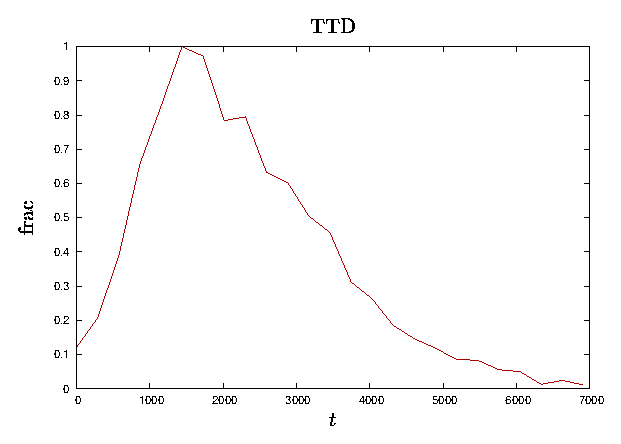
\includegraphics[angle=0,width=10cm]{80_figs/_TTD_0500-0900.eps}
  \caption{Distribution of travel time; $\mu=2404$ s, $\sigma=1270$ s.}
  \label{travtime}
\end{figure}
To generate the distribution of travel times shown in \Figref{travtime}, \\
\comline{java -jar TravelTimeTool.jar TTD 05:00,09:00,16 0,3600,30 madrid\_01.zo }\\
In addition to the `TTD' mode, there are modes which generate synthetic
reference data (`SYN'), compare against reference data (`TTC'),
and evaluate an objective function for calibration (`OBJ').

These modes are described below; they can be demonstrated in sequence by running\\
\comline{./01\_Run\_ZIM\_SYN\_TTD\_TTC\_OBJ.sh}

\section{Synthetic reference data}
To exhibit how calibration can be performed, a reference set of travel
times can be generated, based on a simulation run, with a command like:\\
\comline{java -jar TravelTimeTool.jar SYN 100 out/madrid\_01.zo > \_SYN\_TravelTimeData.csv} \\
The file {\tt \_SYN\_TravelTimeData.csv} produced will be the reference data,
used in here in place of actual ground-truth measurements.

\section{Comparison}
To see the discrepancy between the simulation output and the reference data:
{\tt java -jar TravelTimeTool.jar TTC 05:00,09:00,16 -600,600,20 \_SYN\_TravelTimeData.csv out/madrid\_01.zo }\\
For this example, the time interval between 05:00 and 09:00 is considered.
The result is shown in \Figref{TTdiff}.
\begin{figure}[ht!]
  \centering
  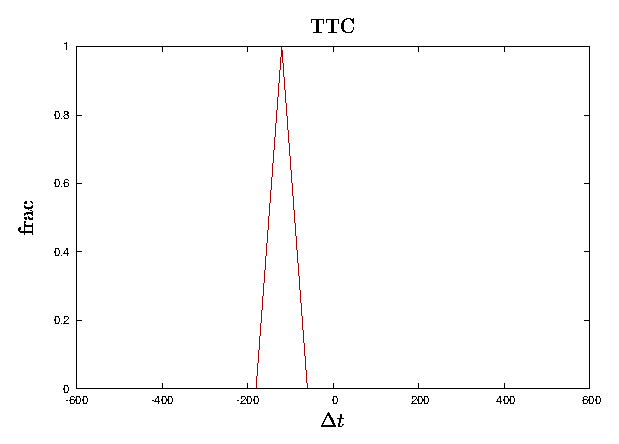
\includegraphics[angle=0,width=10cm]{80_figs/_TTC_0500-0900.eps}
  \caption{Distribution of travel-time error}
  \label{TTdiff}
\end{figure}
This shows that the travel times (compared within `bins' as described before) are 100 seconds
faster than the reference data. (Fluctuations average out, making this distribution very narrow.)
The mean simulation travel-time error is $-100$ s with a standard deviation of $7.37$ s.

\section{Objective}
\label{DefObj}
The parameters of the walking-speed distribution are to be adjusted so that the simulated
travel times correspond as closely as possible to the reference data.
The objective used for this purpose is
\[
\Phi(\mu,\sigma) := \sum_{o,d,\tau} (\tilde{T}_{o,d,\tau} - T_{o,d,\tau})^2
\]
where $\mu$ and $\sigma$ are the mean and standard deviation of the
log-normal distribution\footnote{It is noted that they are not the
 mean and standard deviation of the associated normal distribution; this was described in \Secref{sec:zsource}}
used for walking speeds and specified in the \zobj{zsource} in {\tt 00\_StaticTypes.zim}.
These quantities are each measured in m/s.

$\tau$ labels discrete time intervals during the day; these are statistical bins enabling a definition of \emph{comparable} trips.
Two trips are comparable when they share the same origin $o$, the same destination $d$ and begin
during the same interval $\tau$. The specification {\tt 05:00,09:00,16} in the above commands indicates
that there will be $16$ intervals of $15$ minutes each; in this case $\tau=0\dots15$.

$\tilde{T}_{o,d,\tau}$ is the reference travel-time mean for trips from origin $o$ to
destination $d$ during time interval $\tau$. $T_{o,d,\tau}$ is the mean generated by simulation.

\section{Calibration}
The calibrated values for $\mu$ and $\nu$ are those which minimise $\Phi$.
The method used here to approximate this minimum is a discrete search algorithm which is
analogous to gradient descent;
\[
(\mu,\sigma) = {\textup{LocalMin}(\Phi;\mu_0,\sigma_0)}
\]
with parameters $E=1.075$, $R=0.7$, $s_0=1.0e-8$, $\delta=0.01$, $i_{max}=100$ and initial
estimate $\mu_0=2.0$, $\sigma_0=0.7$.
$\hat{C}$ is set to constrain the parameters within sane
ranges; $1 < \mu < 10$ and $0.05 < \sigma < 1.0$ which are not expected to be saturated.

Each evaluation of $\Phi(\mu,\sigma)$ corresponds to a simulation run;
$\Phi$ depends on the simulation output and the reference data.  The
LocalMin algorithm is as follows.

\begin{itemize}
\item[] {\bf algorithm} $\textup{LocalMin}(f;{\bf x}_0)$ to find ${\bf x}$ near ${\bf x}_0$ which sufficiently\\
  minimises $f(\bf x)$ subject to constraints $\hat{C}$.
  \begin{itemize}
  \item[] {\bf Choose} values for constant parameters:
    \begin{itemize}
    \item[] $E$ --- enthusiasm
    \item[] $R$ --- reluctance
    \item[] $\delta$ --- perturbation
    \item[] $i_{max}$ --- maximum iterations
    \end{itemize}
  \item[] {\bf Set} initial values
    \begin{itemize}
    \item[] ${\bf x} \leftarrow {\bf x}_0$ --- initial guess
    \item[] $s \leftarrow s_0$ --- descent factor
    \item[] $i \leftarrow 0$ --- iteration counter
    \end{itemize}
  \item[] {\bf Loop}:
  \item[] {Evaluate} $f$ to numerically define gradient of $f$ at ${\bf x}$:
    \begin{itemize}
    \item[] Evaluate $f_{base} \leftarrow f({\bf x})$ (or use $f_{new}$ if $i>0$ and last step was enthusiastic) 
    \item[] for $j$ from $1$ to $d$ do
      \begin{itemize}
      \item[] Evaluate $f_j \leftarrow f({\bf x} + \delta \hat {\bf j})$
      \end{itemize}
    \item[] ${\bf g}$ defined by $g_j = (f_j - f_{base})/{\delta}$ is a numerical gradient of $f$ at ${\bf x}$.
    \end{itemize}
  \item[] Use ${\bf g}$ to search for a better ${\bf x}$:
    \begin{itemize}
    \item[] $\Delta{\bf x} \leftarrow s {\bf g}$
    \item[] Tentative new estimate: ${\bf x}' \leftarrow {\bf x} + \Delta{\bf x}$
    \item[] Apply constraints: ${\bf x}' \leftarrow \hat{C} {\bf x}'$
    \item[] if ${\bf x}' = {\bf x}$ then
      \begin{itemize}
      \item[] Quit with result ${\bf x}$
      \end{itemize}
    \item[] Evaluate $f_{new} \leftarrow f({\bf x}')$
    \item[] if $f_{new} < f_0$ then
      \begin{itemize}
      \item[] Update estimate: ${\bf x} \leftarrow {\bf x}'$
      \item[] Exhibit enthusiasm: $ s \leftarrow sE$
      \end{itemize}
    \item[] else if $f_{new} = f_0$ then
      \begin{itemize}
      \item[] Quit with result ${\bf x}$
      \end{itemize}
    \item[] else
      \begin{itemize}
      \item[] Exhibit reluctance: $ s \leftarrow sR$
      \end{itemize}
    \end{itemize}
  \item[] $i \leftarrow i+1$
  \item[] Check:
    \begin{itemize}
    \item[] if $i>i_{max}$ then quit with result ${\bf x}$
    \item[] if $|\Delta{\bf x}| < dx$ then quit with result ${\bf x}$
    \end{itemize}
  \end{itemize}
\end{itemize}
The notation is that ${\bf x}$ is of dimension $d$, and $\hat {\bf j}$ is a unit vector in the $j$ direction, with $j=1\dots d$.

\section{Running calibration}

A script performing the above calibration procedure can be run; the synthetic data generated
with the script described above is used.\\
\comline{./02\_Run\_Zim\_Minimise\_Objective.awk} \\
After some computation, the result can be found in the file {\tt \_00\_StaticTypes.zim}:
\[ % 1.32948   0.162204
  v_\mu = 1.329,  \quad v_\sigma = 0.162
.\]

\section{Calibrated model}

Running again the Travel-Time Tool, \\
\comline{./03\_Run\_TTC\_post\_calib.sh} \\
a comparison bewteen the simulator output and the synthetic
reference data now appears as shown in \Figref{TTdiff2}.
The calibration procedure has reduced the mean travel-time error from $-100$ s to $-19$ s 

\begin{figure}[ht]
  \centering
  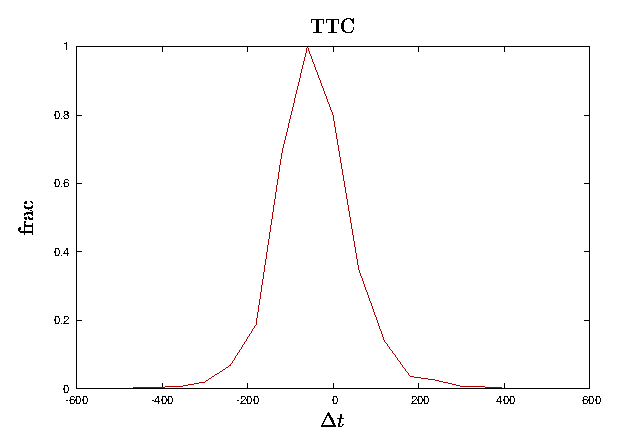
\includegraphics[angle=0,width=10cm]{80_figs/_PostCalib_TTC_0500-0900.eps}
  \caption{Distribution of travel-time error after calibration; $\mu=-15$ s, $\sigma=90$ s.}
  \label{TTdiff2}
\end{figure}

The new global distribution of travel times is shown in the following
chapter, in \Figref{_TTDist2}; it now has a mean of $2333$ s and a
standard deviation of $998$ s.
%\begin{figure}[ht]
%  \centering
%  \includegraphics[angle=0,width=10cm]{_TTD2_0500-2500.eps}
%  \caption{Distribution of travel times after calibration; $\mu=...$ s, $\sigma=...$ s.}  \label{TTglobal2}
%  \label{TTglobal2}
%\end{figure}

In \Chapref{Chap:MadResu} various results will be extracted from the
calibrated simulation.
